% Author: Aurelia Wang
% Email: aureliawang@berkeley.edu
% CSM16A Spring 2023

\begin{center}
    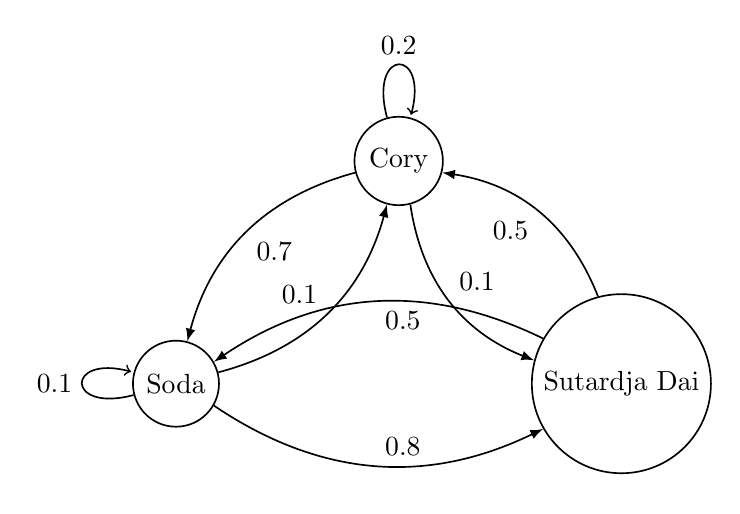
\begin{tikzpicture}[-latex, auto, node distance={4cm}, semithick, main/.style = {draw, circle}]
        \node[main] (Cory) {Cory};
        \node[main, below left of = Cory] (Soda) {Soda};
        \node[main, below right of = Cory] (Sutardja Dai) {Sutardja Dai};
        \path (Cory) edge[loop above] node{0.2} (Cory);
        \path (Cory) edge[bend right] node{0.7} (Soda);
        \path (Cory) edge[bend right] node{0.1} (Sutardja Dai);
        \path (Soda) edge[bend right] node{0.1} (Cory);
        \path (Soda) edge[loop left] node{0.1} (Soda);
        \path (Soda) edge[bend right] node{0.8} (Sutardja Dai);
        \path (Sutardja Dai) edge[bend right] node{0.5} (Cory);
        \path (Sutardja Dai) edge[bend right] node{0.5} (Soda);
    \end{tikzpicture}
\end{center}